\documentclass{book}

\usepackage[utf8]{inputenc}
\usepackage[T1]{fontenc}
\usepackage[francais]{babel}
\usepackage{graphicx} 
\usepackage{adjustbox}
\usepackage{fancyref}
\usepackage{hyperref}
\usepackage{url}


\title{%
  Projet de Sciences des Données \\
  \large Explotation d'images satellites haute-résolution \\pour la prévision d'indicateurs socio-économiques \\
    }

\author{\textsc{Youcef} - \textsc{Kacer}}
\date{22 Septembre 2016}

\begin{document}
 
\maketitle

\tableofcontents

\frontmatter
\chapter{Introduction}
Dans ce document, nous présentons le calcul d'indice végétale par différence normalisée ($NDVI$) lié à une zone géographique. Il est censé renseigner sur la présence de végétaux :
on pense pouvoir utiliser par la suite un tel indicateur afin de prédire et quantifier la densité de population. 

\mainmatter
\chapter{Calcul de l'indice de végétation par différence normalisée (NDVI)}

Cet indice est calculé à partir des canaux
rouge ($R$) et proche-infrarouge ($PIR$) via la formule : 

\[NDVI=\frac{PIR-R}{PIR+R}\]

Typiquement, l'eau, la neige et les nuages refléchissent plus dans le rouge que le proche-infrarouge, soit un $NDVI$ négatif\\
Les sols nus réfléchissent tout autant dans les deux bandes d'où un NDVI nul\\
En revanche, les sols revétus de végétaux refléchissent bien plus dans le proche infra-rouge, ce qui donne un $NDVI$ positif, et d'autant
plus positif que la végétation est dense.\\
Afin de calculer un tel indice sur les images \begin{itshape}Landsat-8\end{itshape}, nous utilisons les bandes géoréférencées $4$ et $5$ 
qui jouent respectivement les r\^oles du rouge (\begin{itshape}0.85-0.88nm\end{itshape}) et du proche-infrarouge (\begin{itshape}0.64-0.67nm\end{itshape}).\\
la librairie $gdal$ sur $python$ nous permet d'effectuer l'opération de différence normalisée sur des rasters pour produire une image de $NDVI$ géoréférencée ($GeoTIFF$).

\begin{figure}[H]
\centerline{
\includegraphics[scale=0.45]{images/Chamonix/08_rgb.png}
\includegraphics[scale=0.45]{images/Chamonix/08_ndvi.png}
\includegraphics[scale=0.4]{images/colormap.png}
}
\begin{center}
\includegraphics[scale=0.45]{images/Chamonix/08_ndvi_histo.png}
\end{center}
\caption{Image couleur, image $NDVI$ et histogramme de $NDVI$ pour la commune de $Chamonix$ sur un périmètre de $116$km2 au mois d'$Aout$}
\label{chamonix_ndvi}
\end{figure}

La figure \ref{chamonix_ndvi} montre un $NDVI$ négatif au sud de la commune de Chamonix, ce qui correspond au glaciers du \begin{itshape}Mont-Blanc\end{itshape}\\

\clearpage 

\begin{figure}[H]
\centerline{
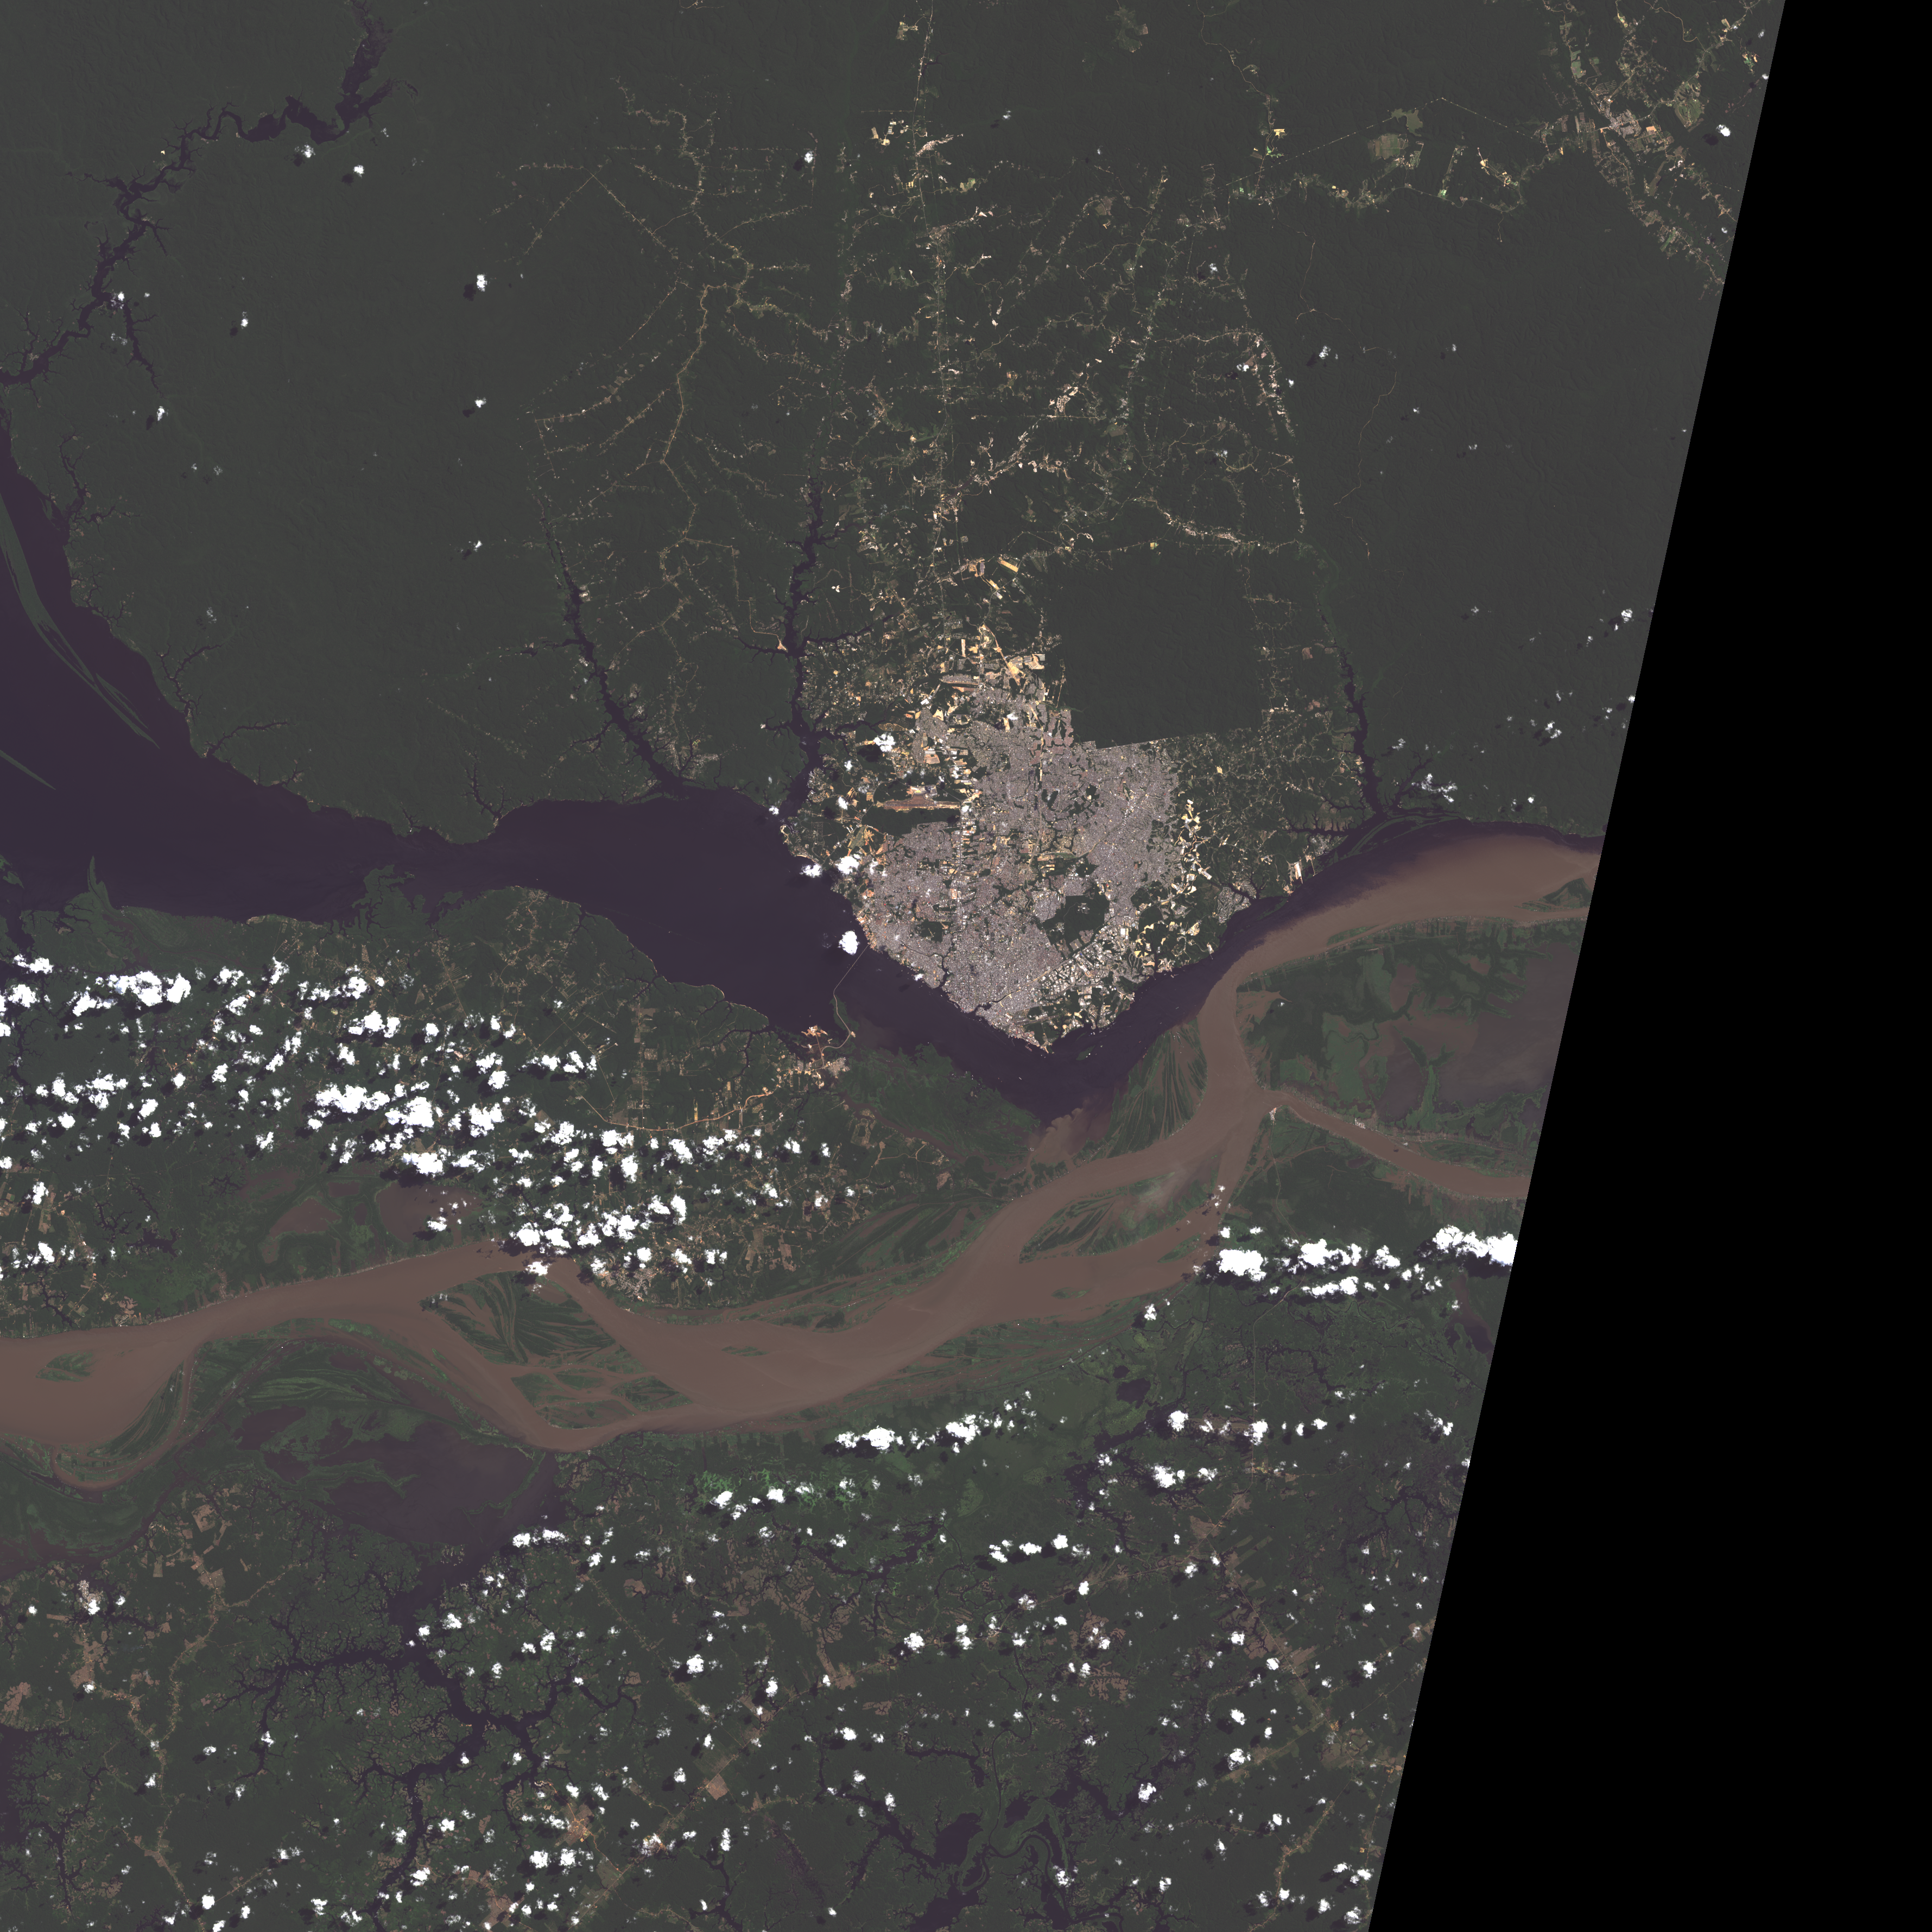
\includegraphics[scale=0.045]{images/Manaus/07_rgb.png}
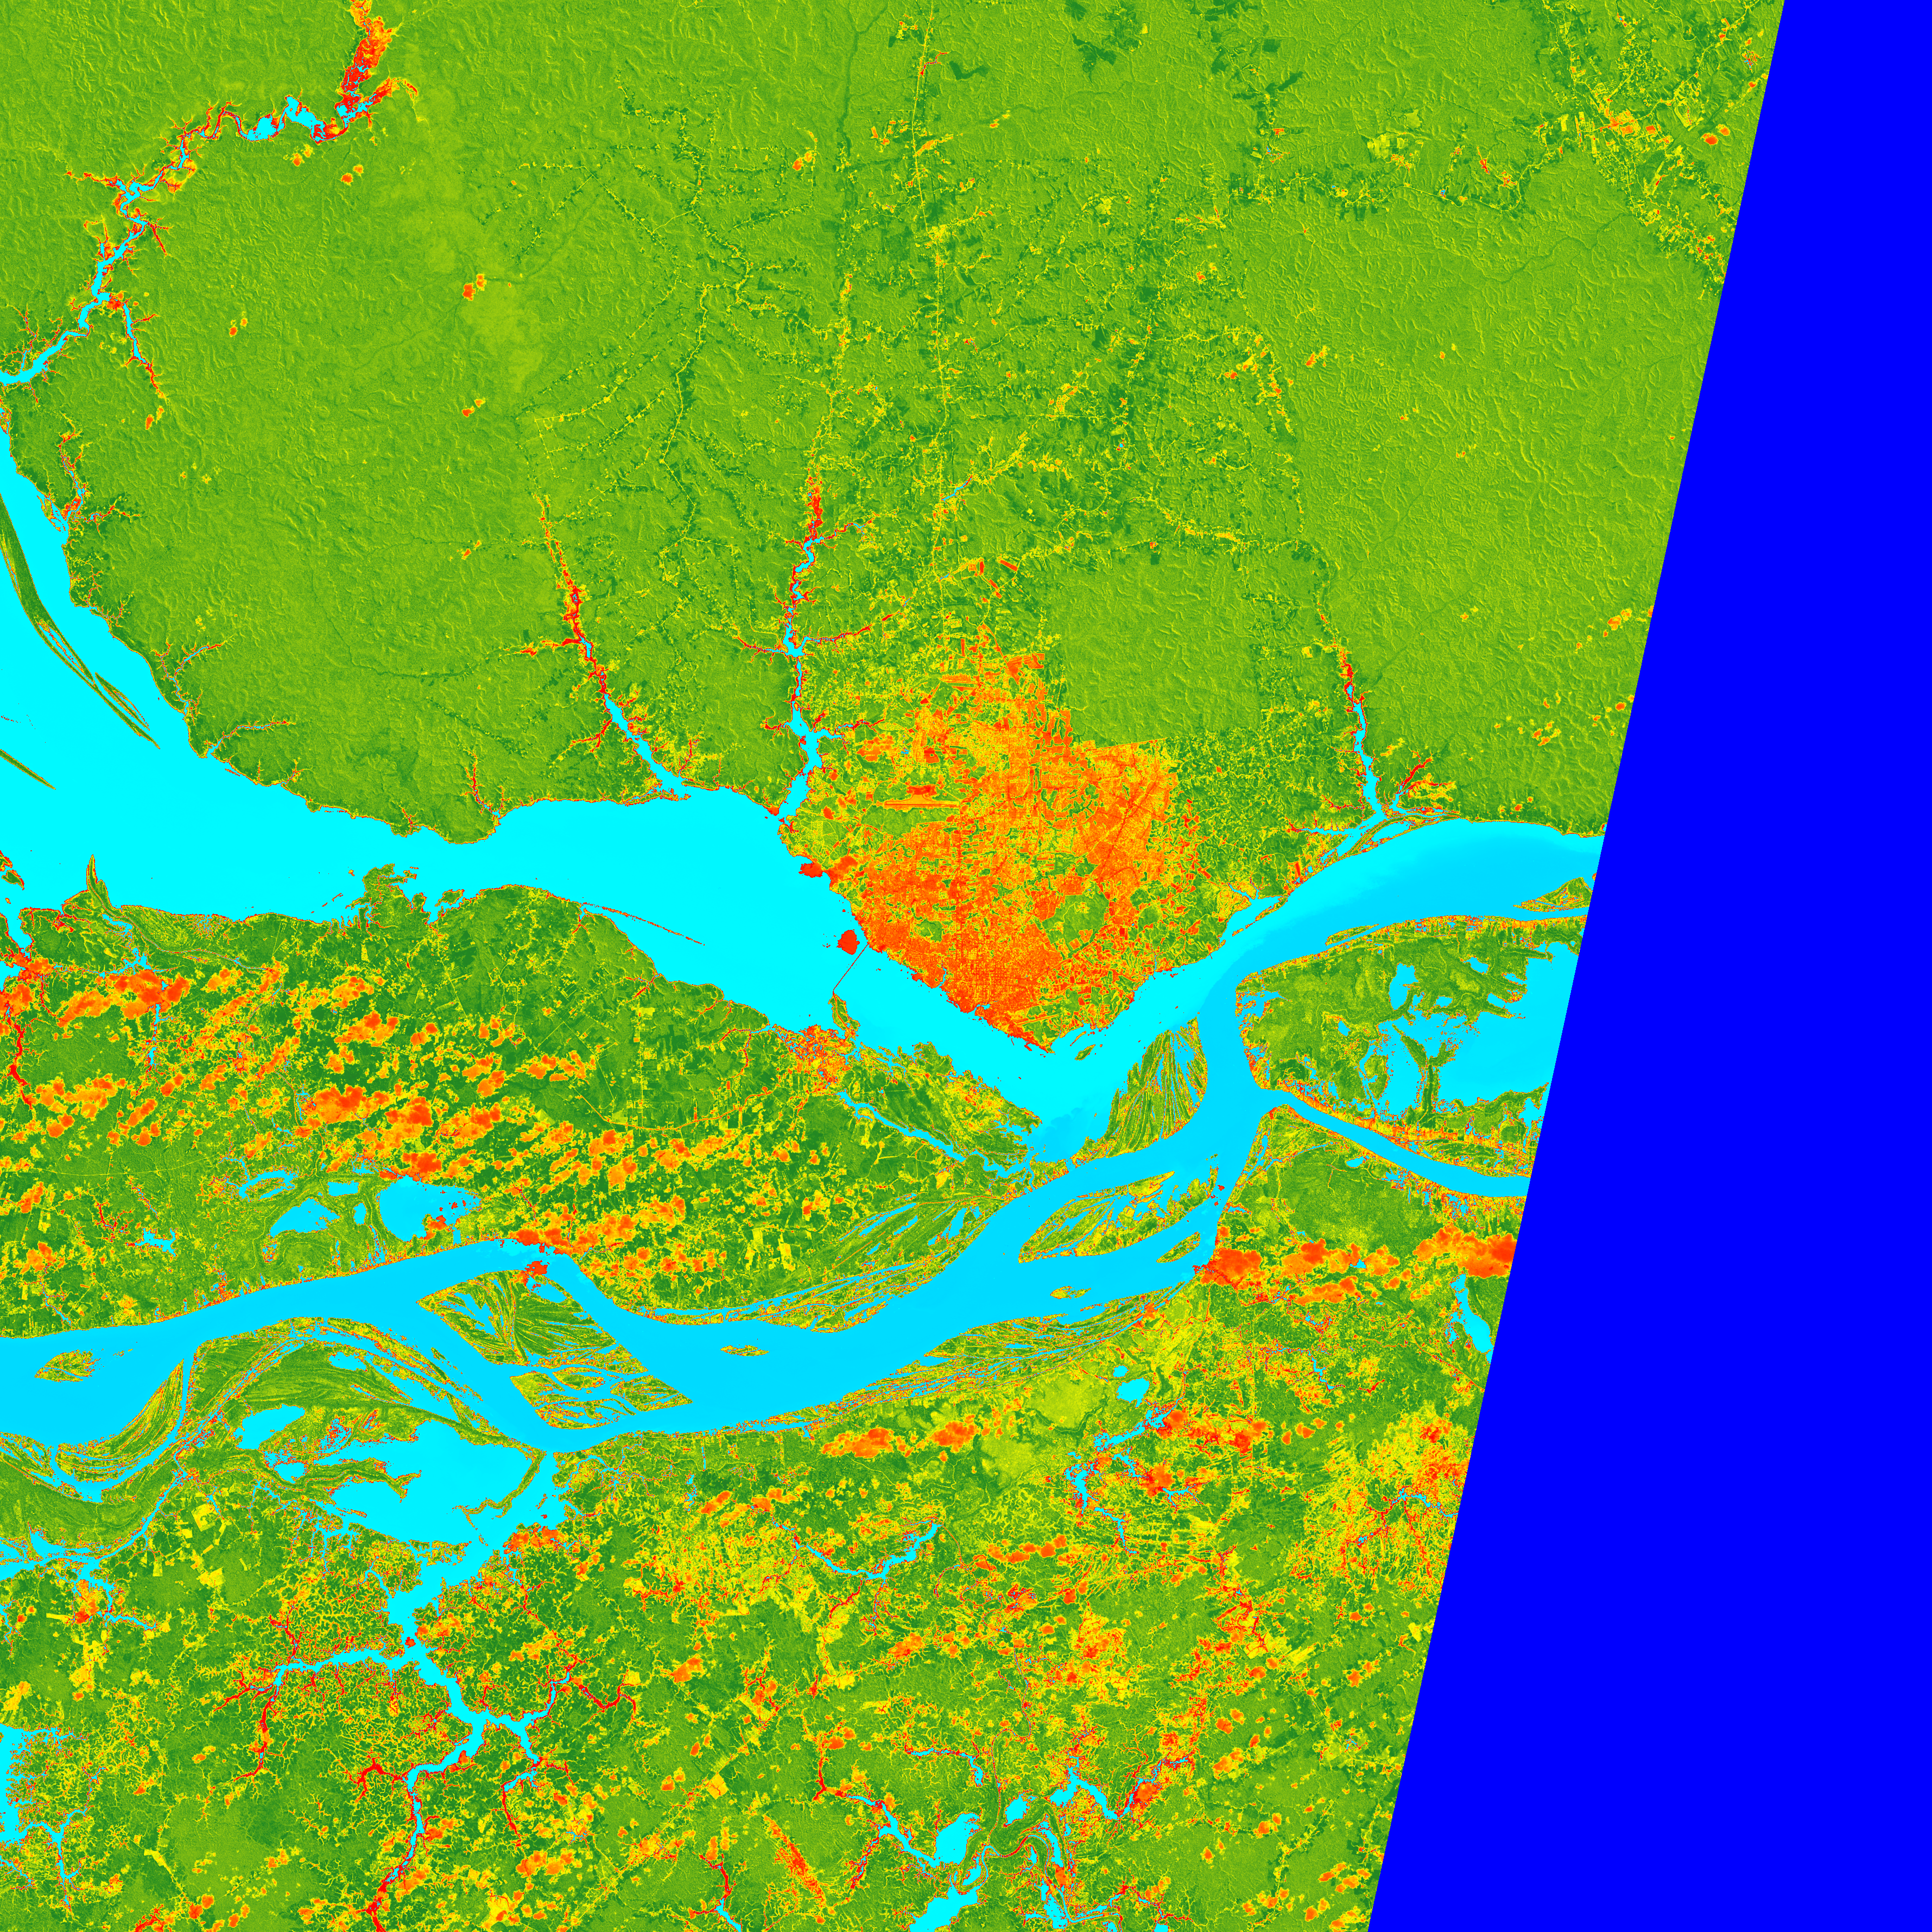
\includegraphics[scale=0.045]{images/Manaus/07_ndvi.png}
\includegraphics[scale=0.4]{images/colormap.png}
}
\begin{center}
\includegraphics[scale=0.45]{images/Manaus/07_ndvi_histo.png}
\end{center}
\caption{Image couleur, image $NDVI$ et histogramme de $NDVI$ pour la ville de $Manaus$ ($Bresil$) sur un périmètre de $11000$km2 au mois de $Juillet$}
\label{manaus_ndvi}
\end{figure}

La figure \ref{manaus_ndvi} montre un $NDVI$ supérieur à $0.5$ autour de la ville de Manaus au Brésil, ce qui correspond à la végétation dense de la for\^et amazonienne. Le fleuve
du \begin{itshape}Rio Negro\end{itshape} apparait lui en négatif\\

\clearpage

\begin{figure}[H]
\centerline{
\includegraphics[scale=0.45]{images/Paris/12_rgb.png}
\includegraphics[scale=0.45]{images/Paris/12_ndvi.png}
\includegraphics[scale=0.4]{images/colormap.png}
}
\begin{center}
\includegraphics[scale=0.4]{images/Paris/12_ndvi_histo.png}
\end{center}
\caption{Image couleur, image $NDVI$ et histogramme de $NDVI$ pour la ville de $Paris$ sur un périmètre de $105$km2 au mois de $Decembre$}
\label{paris_ndvi}
\end{figure}

La figure \ref{paris_ndvi} montre un $NDVI$ quasi nulle donc sans végétation, comme on peut s'y attendre dans une commune urbaine telle que Paris en période hivernale\\

\clearpage


\chapter{Evolution du NDVI au cours d'une année}

Comme vu au chapître précédent, la distribution du $NDVI$ dépend de la présence ou non de végétaux. Ainsi, on peut légitimement se demander comment évolue 
cet indice en fonction des saisons.\\
La figure \ref{paris_ndvi_annee} montre l'évolution du $NDVI$ sur 10 mois pour la ville de $Paris$. On note un étalement de la distribution dans les mois chauds d\^u à l'abondance de végétation à cette époque
de l'année.
\begin{figure}[H]
\centerline{
\includegraphics[scale=0.25]{images/Paris/03_ndvi.png}
\includegraphics[scale=0.2]{images/colormap.png}
\includegraphics[scale=0.25]{images/Paris/04_ndvi.png}
\includegraphics[scale=0.2]{images/colormap.png}
\includegraphics[scale=0.25]{images/Paris/05_ndvi.png}
\includegraphics[scale=0.2]{images/colormap.png}
\includegraphics[scale=0.25]{images/Paris/06_ndvi.png}
\includegraphics[scale=0.2]{images/colormap.png}
\includegraphics[scale=0.25]{images/Paris/07_ndvi.png}
\includegraphics[scale=0.2]{images/colormap.png}
}
\centerline{
\includegraphics[scale=0.25]{images/Paris/08_ndvi.png}
\includegraphics[scale=0.2]{images/colormap.png}
\includegraphics[scale=0.25]{images/Paris/09_ndvi.png}
\includegraphics[scale=0.2]{images/colormap.png}
\includegraphics[scale=0.25]{images/Paris/10_ndvi.png}
\includegraphics[scale=0.2]{images/colormap.png}
\includegraphics[scale=0.25]{images/Paris/11_ndvi.png}
\includegraphics[scale=0.2]{images/colormap.png}
\includegraphics[scale=0.25]{images/Paris/12_ndvi.png}
\includegraphics[scale=0.2]{images/colormap.png}
}
\begin{center}
\includegraphics[scale=0.45]{images/Paris/all_ndvi_histo.png}
\end{center}
\caption{De la gauche vers la droite sur la première ligne, évolution du $NDVI$ entre $Mars$ et $Juillet$ pour la ville de $Paris$ sur un périmètre de $105$km2.
De la gauche vers la droite sur la seconde ligne, évolution du $NDVI$ entre $Aout$ et $Decembre$ pour la ville de $Paris$ sur un périmètre de $105$km2. 
En bas, supersposition des histogrammes de $NDVI$ pour les mois de $Mars$ à $Decembre$}
\label{paris_ndvi_annee}
\end{figure}

\clearpage

Cette différence est encore plus nette pour une ville moins urbaine comme $Fontainebleau$ \ref{fontainebleau_ndvi_annee}.
 
\begin{figure}[H]
\centerline{
\includegraphics[scale=0.25]{images/Fontainebleau/03_ndvi.png}
\includegraphics[scale=0.2]{images/colormap.png}
\includegraphics[scale=0.25]{images/Fontainebleau/04_ndvi.png}
\includegraphics[scale=0.2]{images/colormap.png}
\includegraphics[scale=0.25]{images/Fontainebleau/05_ndvi.png}
\includegraphics[scale=0.2]{images/colormap.png}
\includegraphics[scale=0.25]{images/Fontainebleau/06_ndvi.png}
\includegraphics[scale=0.2]{images/colormap.png}
\includegraphics[scale=0.25]{images/Fontainebleau/07_ndvi.png}
\includegraphics[scale=0.2]{images/colormap.png}
}
\centerline{
\includegraphics[scale=0.25]{images/Fontainebleau/08_ndvi.png}
\includegraphics[scale=0.2]{images/colormap.png}
\includegraphics[scale=0.25]{images/Fontainebleau/09_ndvi.png}
\includegraphics[scale=0.2]{images/colormap.png}
\includegraphics[scale=0.25]{images/Fontainebleau/10_ndvi.png}
\includegraphics[scale=0.2]{images/colormap.png}
\includegraphics[scale=0.25]{images/Fontainebleau/11_ndvi.png}
\includegraphics[scale=0.2]{images/colormap.png}
\includegraphics[scale=0.25]{images/Fontainebleau/12_ndvi.png}
\includegraphics[scale=0.2]{images/colormap.png}
}
\begin{center}
\includegraphics[scale=0.45]{images/Fontainebleau/all_ndvi_histo.png}
\end{center}
\caption{De la gauche vers la droite sur la première ligne, évolution du $NDVI$ entre $Mars$ et $Juillet$ pour la ville de $Fontainebleau$ sur un périmètre de $172$km2.
De la gauche vers la droite sur la seconde ligne, évolution du $NDVI$ entre $Aout$ et $Decembre$ pour la ville de $Fontainebleau$ sur un périmètre de $172$km2. 
En bas, supersposition des histogrammes de $NDVI$ pour les mois de $Mars$ à $Decembre$}
\label{fontainebleau_ndvi_annee}
\end{figure}

On note donc que le $NDVI$ au saison chaude permet de mieux discriminer les villes très urbabnisées comme $Paris$ des communes plus rurales comme $Fontainebleau$. En effet, il y a apparition
d'un mode princpal à haute fréquence dans le second cas que l'on n'observe pas dans le premier.
\clearpage

\backmatter

\listoftables

\listoffigures

\bibliographystyle{alpha}
\bibliography{biblio}

\end{document}